\documentclass[conference]{IEEEtran}

\usepackage{cite}
\ifCLASSINFOpdf
\usepackage[pdftex]{graphicx}
\graphicspath{{../script/fig/}{./figures/}}
\DeclareGraphicsExtensions{.pdf,.jpeg,.png, .jpg, .PNG}
\else
\fi
\usepackage{amsmath,bm}
\interdisplaylinepenalty=2500
\ifCLASSOPTIONcompsoc
\usepackage[caption=false,font=normalsize,labelfont=sf,textfont=sf]{subfig}
\else
\usepackage[caption=false,font=footnotesize]{subfig}
\fi
\usepackage{url}
\usepackage{amsfonts} % for \mathbb{}
\usepackage{listings} % For writing math in verbatim
\usepackage{enumerate}

\usepackage[showlabels,sections,floats,textmath,displaymath]{preview}
\usepackage{amssymb} %% For showing special symbols like \bigstar
\usepackage{pifont}  %% For showing circled numbers
\usepackage{array}
%\usepackage{algorithm}
\usepackage{algpseudocode}
\usepackage{ifthen}
\usepackage{dirtree}
%\setlength{\DTbaselineskip}{13pt}
%\renewcommand*\DTstyle{}
%\DTsetlength{.2em}{1em}{.2em}{.4pt}{2pt}

\newcommand{\mathnew}{\mathit} 
% for nice reference 
\newcommand{\fsp}{{\;}}
\newcommand{\Fig}{\figurename \fsp}
\newcommand{\Sec}{Sec.\fsp}
\newcommand{\Eq}{Eq.\fsp}
\newcommand{\Tab}{Tab.\fsp}
\newcommand{\Alg}{Alg.\fsp}

\DeclareMathOperator*{\argminB}{argmin} 

\hyphenation{temperature} % correct bad hyphenation here

\usepackage{tikz}
\usetikzlibrary{arrows}
\usetikzlibrary{intersections}
\usetikzlibrary{calc, quotes}
\usetikzlibrary{external}
\tikzexternalize[prefix=tikz_figures/]%
\pgfdeclarelayer{bg}    % declare background layer
\pgfsetlayers{bg,main} % set the order of the layers (main is the standard layer)
\usetikzlibrary{patterns}

\newcommand{\etal}{\textit{et al}. }
\newcommand{\ie}{\textit{i}.\textit{e}. }
\newcommand{\eg}{\textit{e}.\textit{g}. }

%%
%% Check this post for how to write properly-sized ceiling operator
%% https://tex.stackexchange.com/a/367035/172530
%%
\usepackage{mathtools}
\DeclarePairedDelimiter{\ceil}{\lceil}{\rceil}

%% For text color
\usepackage{xcolor}

%% For drawing boxes around text
%% https://tex.stackexchange.com/a/234195/172530
\newcommand\textbox[2]{%
  \tikz[baseline]\node[%
  inner ysep=0pt, 
  inner xsep=2pt, 
  anchor=text, 
  rectangle, 
  rounded corners=1mm,
  #1] {\strut#2};%
}

%% package for highlighting text
%% Usage: \hl{text to be highlighted}
\usepackage{soul}
\sethlcolor{yellow}

%% underlining for emphasis
%% Examples:
%% \uline{important} underline
%% \uuline{urgent} double-underline
%% \uwave{boat} wavy underline like
%% \sout{wrong} line struck through word
%% \xout{removed} removed
%% \dashuline{dashing} dashed
%% \dotuline{dotty} dotted
\usepackage[normalem]{ulem}

%% define a red check mark
\newcommand\redcheck{
  {\textcolor{red}{\ding{52}}}
}

\usepackage{dblfloatfix}    % To enable figures at the bottom of page

\usepackage{wrapfig}
\usepackage{siunitx}

% Overlay question mark on equal mark
\def\qeq{\mathrel{%
    \mathchoice{\QEQ}{\QEQ}{\scriptsize\QEQ}{\tiny\QEQ}%
}}
\def\QEQ{{%
    \setbox0\hbox{=}%
    \rlap{\hbox to \wd0{\hss?\hss}}\box0
  }}


%% Enabling this package will automatically align the text in the two columns vertically
%\usepackage{widetext}


%% https://tex.stackexchange.com/questions/2441/how-to-add-a-forced-line-break-inside-a-table-cell
\usepackage{makecell} %% For breaking lines in table cells

\usepackage{amsthm}
\theoremstyle{definition}
\newtheorem{definition}{Definition}

\theoremstyle{proposition}
\newtheorem{proposition}{Proposition}

\DeclareMathOperator*{\argmax}{arg\,max}
\DeclareMathOperator*{\argmin}{arg\,min}

%% It is tricky to use the algorithm2e package in the ieeetran document
%% Check this post for tweaks
%% https://tex.stackexchange.com/a/147625
\usepackage[ruled,norelsize,linesnumbered, vlined, longend]{algorithm2e}
\makeatletter
\newcommand{\removelatexerror}{\let\@latex@error\@gobble}
\makeatother


\begin{document}

\title{Implementation of Monte Carlo Localization on Heterogeneous Platform}

\author{\IEEEauthorblockN{Lixun Zhang, Aloysius K. Mok
\IEEEauthorblockA{Department of Computer Science\\
University of Texas at Austin,
Austin, Texas}}}

\maketitle

\begin{abstract}
  This report summarizes the experiment results of different implementations of
  the Monte Carlo Localization (MCL) algorithm.
\end{abstract}

\section{Introduction}

Localization solves the following problem:

\begin{quote}
  Given a map and sensor data, estimate the position and orientation of the robot.
\end{quote}

Monte Carlo Localization (MCL) solves the localization problem using particle
filter.

\section{The Monte Carlo Localization Algorithm}
MCL is a recursive Bayes filter that estimates the posterior distribution of robot
poses conditioned on sensor data.
Bayes filters address the problem of estimating the state x of a dynamical system
(partially observable Markov chain) from sensor measurements.

Details of the mathematical foundation of MCL can be found in \cite{THRUN200199}.

\section{The Implementation of MCL}

\subsection{Implementation of the \texttt{motion\_model}}
\subsection{Implementation of the \texttt{sensor\_model}}

\subsection{Implementation of the \texttt{Resampling} Algorithm}

\subsection{Multi-threading Implementation on CPU}

\subsection{CUDA Implementation on GPU}

\subsection{Hybrid Implementation on CPU+GPU}


\section{Experiment Setup}
The MCL algorithm is implemented as a node in the ROS environment, which also
launches the following nodes:
\begin{itemize}
\item The map server, which loads the map for localization.
  For all experiments, the 2D occupancy grid map of MIT basement is used, which
  is shown in \Fig \ref{fig:omap}.
\item The car model, which describes the robot car and publishes robot state
\item rosbag, which replays the laser range sensor data and odometry recorded
  in a previous run of the robot car in a simulation environment.
\item rviz, which is used for visualization.
\end{itemize}

\begin{figure}[!h]
  \centering 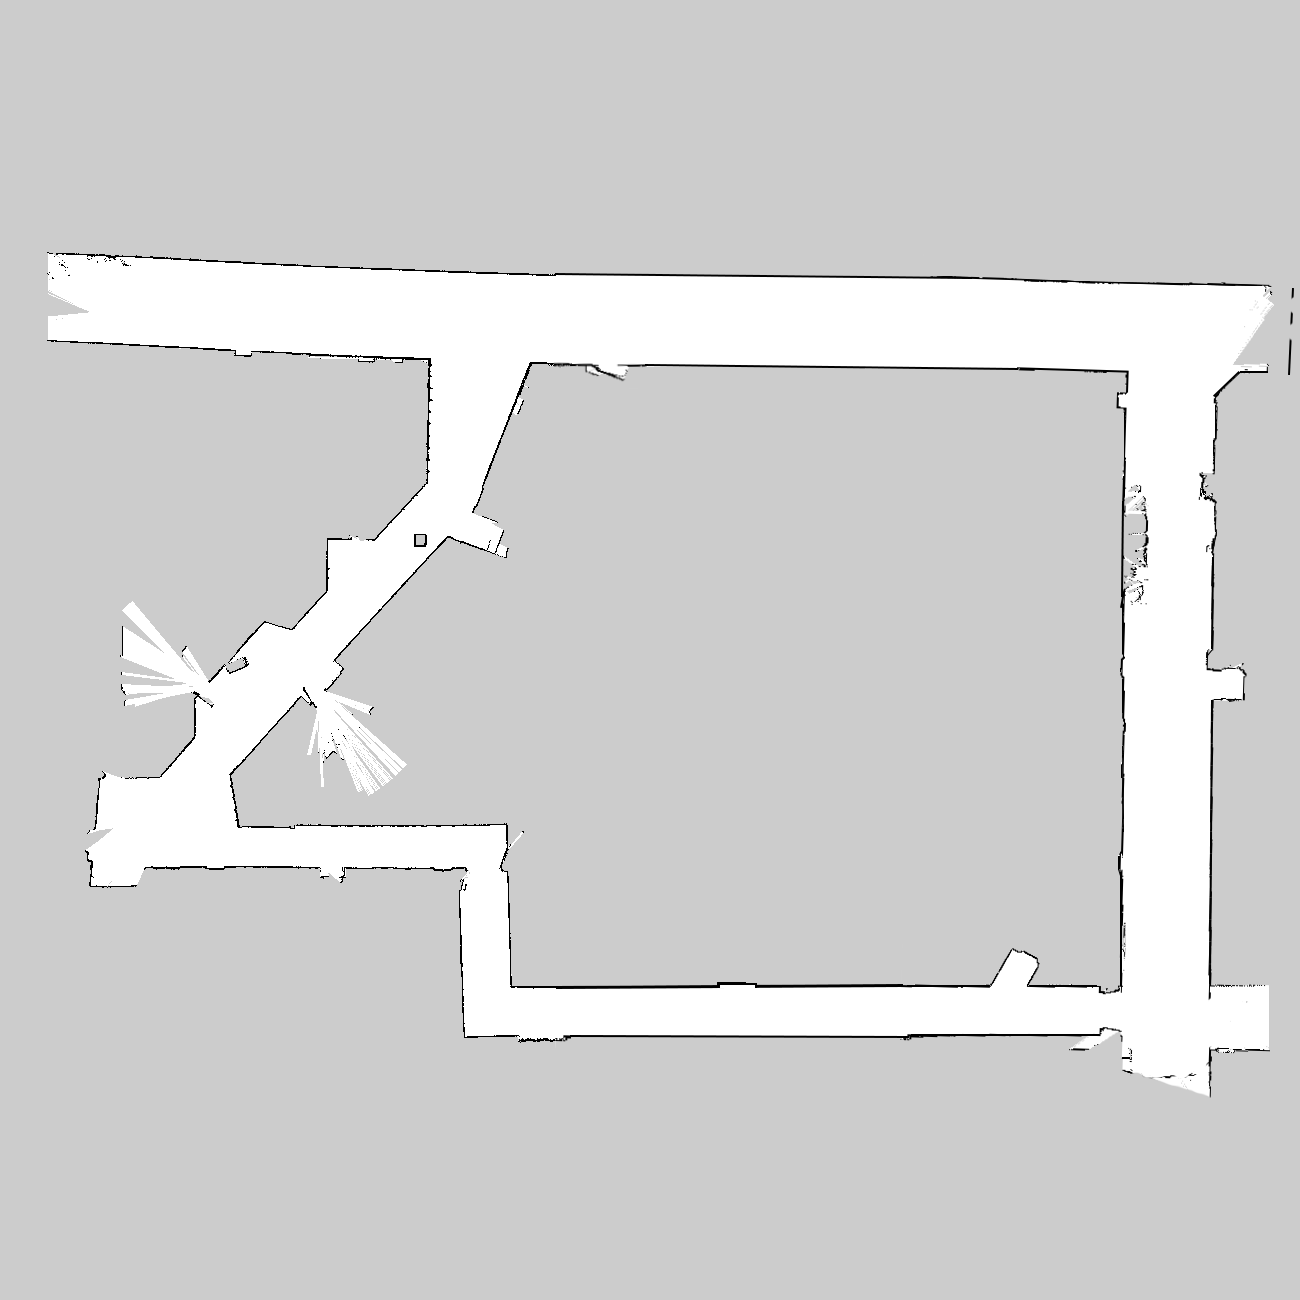
\includegraphics[width=.5\linewidth]{basement_fixed.png}
  \caption{The 2D occupancy grid map used in the experiment.}
  \label{fig:omap}
\end{figure}

\section{Experiment Results}
\subsection{Robot Localization Accuracy}

\Fig \ref{fig:demo} illustrates 4 screenshots, corresponding to 4 situations
during the simulation.
The robot car is represented by the small blue rectangle in the middle of the
figure. Red arrows are particles and the long blue arrow is the pose estimate
from the MCL algorithm.

\begin{figure}[!h]
  \subfloat[multiple false estimates]{
    \centering \includegraphics[width=0.47\linewidth]{false_local}
    \label{fig:demoa}}
  \hfil
  \subfloat[single false estimate]{
    \centering \includegraphics[width=.47\linewidth]{false_local1}
    \label{fig:demob}}
  \hfil
  \subfloat[no estimate]{
    \centering \includegraphics[width=0.47\linewidth]{fail}
    \label{fig:democ}}
  \hfil
  \subfloat[good tracking]{
    \centering \includegraphics[width=.47\linewidth]{success1}
    \label{fig:demod}}
  \caption{Demonstration of robot localization in rviz.}
  \label{fig:demo}
\end{figure}

\Fig \ref{fig:demoa} shows the situation where the particles fall into three
regions, but none of them captures the true pose of the robot.
\Fig \ref{fig:demob} shows that the particles fall into the same area, which
is not a correct estimate of the robot pose.
\Fig \ref{fig:democ} shows the situation where particles are not converging yet.
This is because all particles are not likely to be the true state, thus having
negligible weights.
\Fig \ref{fig:demod} shows the situation of a good tracking.
The pose of the robot is correctly computed by the particles and the estimate
evolves along with the motion of the robot.

The visualization in rivz makes it clear whether the particles tracks the robot,
but it is difficult, if possible, to analyze the accuracy of the localization.
Therefore, we have done experiments with different number of particles and
various confidence of the initial position of the robot in the map.
The results are shown in \Fig \ref{fig:maxW}.


\begin{figure}[!h]
  \subfloat[Effect of number of particles]{
    \centering \includegraphics[width=.47\linewidth]{averaged_maxW}
    \label{fig:averaged_maxW}}
  \hfil
  \subfloat[Effect of init pose confidence]{
    \centering \includegraphics[width=.47\linewidth]{maxW_error}
    \label{fig:maxW_error}}
  \caption{Localization accuracy with difference configurations.
    A black horizontal line at maxW=18.5 is drawn as the threshold above which the
    particles are considered as tracking the robot correctly.
    (a) The maximum particle weight of 1000 iterations of the MCL algorithm
    using different number of particles. Each value is averaged among 10
    individual experiments of the same configuration. The confidence of the
    initial pose of the robot is low.
    (b) The maximum particle weight of different number of particles with high,
    medium, and low confidence about the initial pose of the robot. The value is
    first averaged along all the iterations for each individual experiment. Then
    the averaged value is further averaged among 10 individual experiments.}
  \label{fig:maxW}
\end{figure}

%%
%% Explanation of the metric: dis, maxW, and diffW
%%
Before diving into the experiment results, we need to explain the metric used to
evaluate the quality of the localization.
There are some candidates:
\begin{itemize}
\item Euler distance between the estimated pose and the true pose.
  This metric is simple to implement but it ignores the orientation of the robot.
  We found that when the particles are tracking the robot, the distance between
  the estimated pose and the true pose is always smaller than 0.3 m.
  This metric is not used as the evaluation of MCL's accuracy, but it is used to
  determine whether resampling should be performed for the next iteration.
\item Maximum weight\footnote{
    Actually, maxW is computed from the maximum weight by
    $\log_{10}(w) \text{+} 63$ because the raw weight computed by the sensor
    model is too close to zero, which is hard to compare and visualize.
  } (maxW) among all particles.
  Since the weight of each particle is computed by the sensor model, the maxW
  indicates the weight of the most likely particle.
  If maxW is good enough, then the particles should be able to track the robot.
  If maxW is too small, none of the particles is close enough to the true state.
  This metric is used to evaluate the accuracy of MCL and it is the label of
  y-axis in \Fig \ref{fig:maxW}.
\item The weight of the estimated pose (diffW) computed by the sensor model.
  If the estimated pose is computed as the particles with the maximum weight,
  diffW and maxW are the same.
  We also observe that diffW and maxW are very close when other expectation
  methods are used.
  Since maxW is used as the metric, using diffW will not provide more information
  about the accuracy of MCL.
\end{itemize}

%%
%% Explanation of the confidence level
%%
The confidence of the initial pose refers to how much knowledge we have about
the initial pose of the robot at the beginning.
This is modeled as the standard deviation of the 2D Gaussian distribution when
initializing the particles.
The particles are initialized by the Gaussian distribution centered at (0,0) in
the map, which is the true starting point of the robot.
The orientations of the particles are sampled uniformly in the range of 0 to 2$\pi$.
The high, medium, and low confidence correspond to the standard deviation values
of 1, 3, and 5.

%%
%% Explanation of accuracy experiment results
%%
\Fig \ref{fig:averaged_maxW} compares the accuracy of MCL when using different
numbers of particles.
The localization accuracy increases as iterations go.
We have the following observations:
\begin{itemize}
\item When insufficient number of particles are used (\eg when n=100), the pose
  of the robot is not tracked.
\item When more particles are used (\eg when n=1000), MCL locates the robot after
  about 300 iterations.
  But it loses the robot after about 450 iteration.
  Then it locates the robot again at about 700 iterations and loses it again at
  about 850 iterations.
  In this case, the tracking capability of MCL is unstable and depends on the
  initial guess and map information.
\item When sufficient number of particles (\eg when n=5120 and n=10240), MCL is
  able to track the robot from about the 50th iteration to the end.
  The benefit of using 10240 particles is that the accuracy increases faster at
  the beginning, i.e. it takes shorter time for MCL to locate the robot.
\end{itemize}

\Fig \ref{fig:maxW_error} compares the accuracy of MCL when different confidence
is used to initialize the particles.
The difference is more obvious when insufficient number of particles is used.
When the number of particles is larger than 4000, the tracking capability of MCL
is robust regardless of the confidence level of the initial particles.


\subsection{Timing Results on Heterogeneous Platforms}


\begin{figure}[!h]
  \subfloat[Self-built machine]{
    \centering \includegraphics[width=.47\linewidth]{TITAN_MT_time}
    \label{fig:titan_mt_time}}
  \hfil
  \subfloat[Jetson TX2]{
    \centering \includegraphics[width=.47\linewidth]{jetson_MT_time}
    \label{fig:jetson_mt_time}}
  \caption{Elapsed time per MCL iteration with different implementations.
    The black horizontal line refers to the message processing deadline of
    \SI{10}{\ms}, \ie \SI{100}{\hertz}.
    mt=n means n threads are used to execute the \texttt{update} part of MCL
    in parallel.}
  \label{fig:compare_cpu_gpu}
\end{figure}

\Fig \ref{fig:compare_cpu_gpu} shows the averaged elapsed time of one MCL iteration
on CPU with different levels of multi-threading and GPU.
The goal is to finish one iteration of MCL within \SI{10}{\ms} due to the message
publishing rate of \SI{100}{\hertz}.
It can be seen from the figure that GPU implementation is much faster than its CPU
counterpart, even thought multiple threads are working in parallel in the CPU
implementation.
The same behavior can be observed on both the self-built machine
(\Fig \ref{fig:titan_mt_time}) and the Jetson TX2 platform
(\Fig \ref{fig:jetson_mt_time}).


\begin{figure}[!h]
  \subfloat[Self-built machine]{
    \centering \includegraphics[width=.47\linewidth]{TITAN_component_timing}
    \label{fig:titan_component_timing}}
  \hfil
  \subfloat[Jetson TX2]{
    \centering \includegraphics[width=.47\linewidth]{jetson_component_timing}
    \label{fig:jetson_component_timing}}
  \caption{Elapsed time of each component of MCL with different implementations.
    (a) mt=7 (b) mt=5}
  \label{fig:component_timing}
\end{figure}

\Fig \ref{fig:component_timing} shows the elapsed time of each component of MCL.
As can be seen, the most time consuming part of MCL is the \texttt{update} function,
which includes \texttt{motion\_model} and \texttt{sensor\_model}.


\begin{figure}[!h]
  \subfloat[Self-built machine]{
    \centering \includegraphics[width=.47\linewidth]{TITAN_hybrid_timing}
    \label{fig:titan_hybrid_timing}}
  \hfil
  \subfloat[Jetson TX2]{
    \centering \includegraphics[width=.47\linewidth]{jetson_hybrid_timing}
    \label{fig:jetson_hybrid_timing}}
  \caption{Elapsed time of the \texttt{update} part of MCL by the hybrid implementation.
    For each n, different combinations of $\text{n}_c$ and $\text{n}_g$ are used
    and the best result is plotted as the hybrid line in the figures, where
    $\text{n}_c$ is the number of particles assigned to CPU and $\text{n}_g$ is
    the number of particles assigned to GPU.
    (a) mt=7 (b) mt=5}
  \label{fig:hybrid_timing}
\end{figure}

\Fig \ref{fig:hybrid_timing} shows the averaged elapsed time of \texttt{update}
function implemented on CPU and GPU in a hybrid manner.
It can be seen that using the hybrid implementation yields almost the same
performance as the GPU implementation.
This means that partitioning particles among CPU and GPU does not improve the
performance.
This is because the difference between CPU and GPU is so huge that assigning
a good number of  particles to CPU will lead to the elapsed time of the
\texttt{update} function exceeds the deadline.
But assigning few particles to CPU has negligible effects on the elapsed time
of the GPU implementation.


\bibliographystyle{IEEEtran}
\bibliography{/home/lixun/Dropbox/PhD/lit_review/lit_review.bib}
\end{document}
%%% Local Variables:
%%% TeX-command-extra-options: "-shell-escape"
%%% mode: latex
%%% TeX-master: t
%%% End:
